\chapter*{Numerical grids}
We distinguish two types of numerical grids: the 3D soil grid and the 1D, branched, root system grid (see Fig. \ref{fig:grids}). 

\begin{figure}[ht]
	\centering
  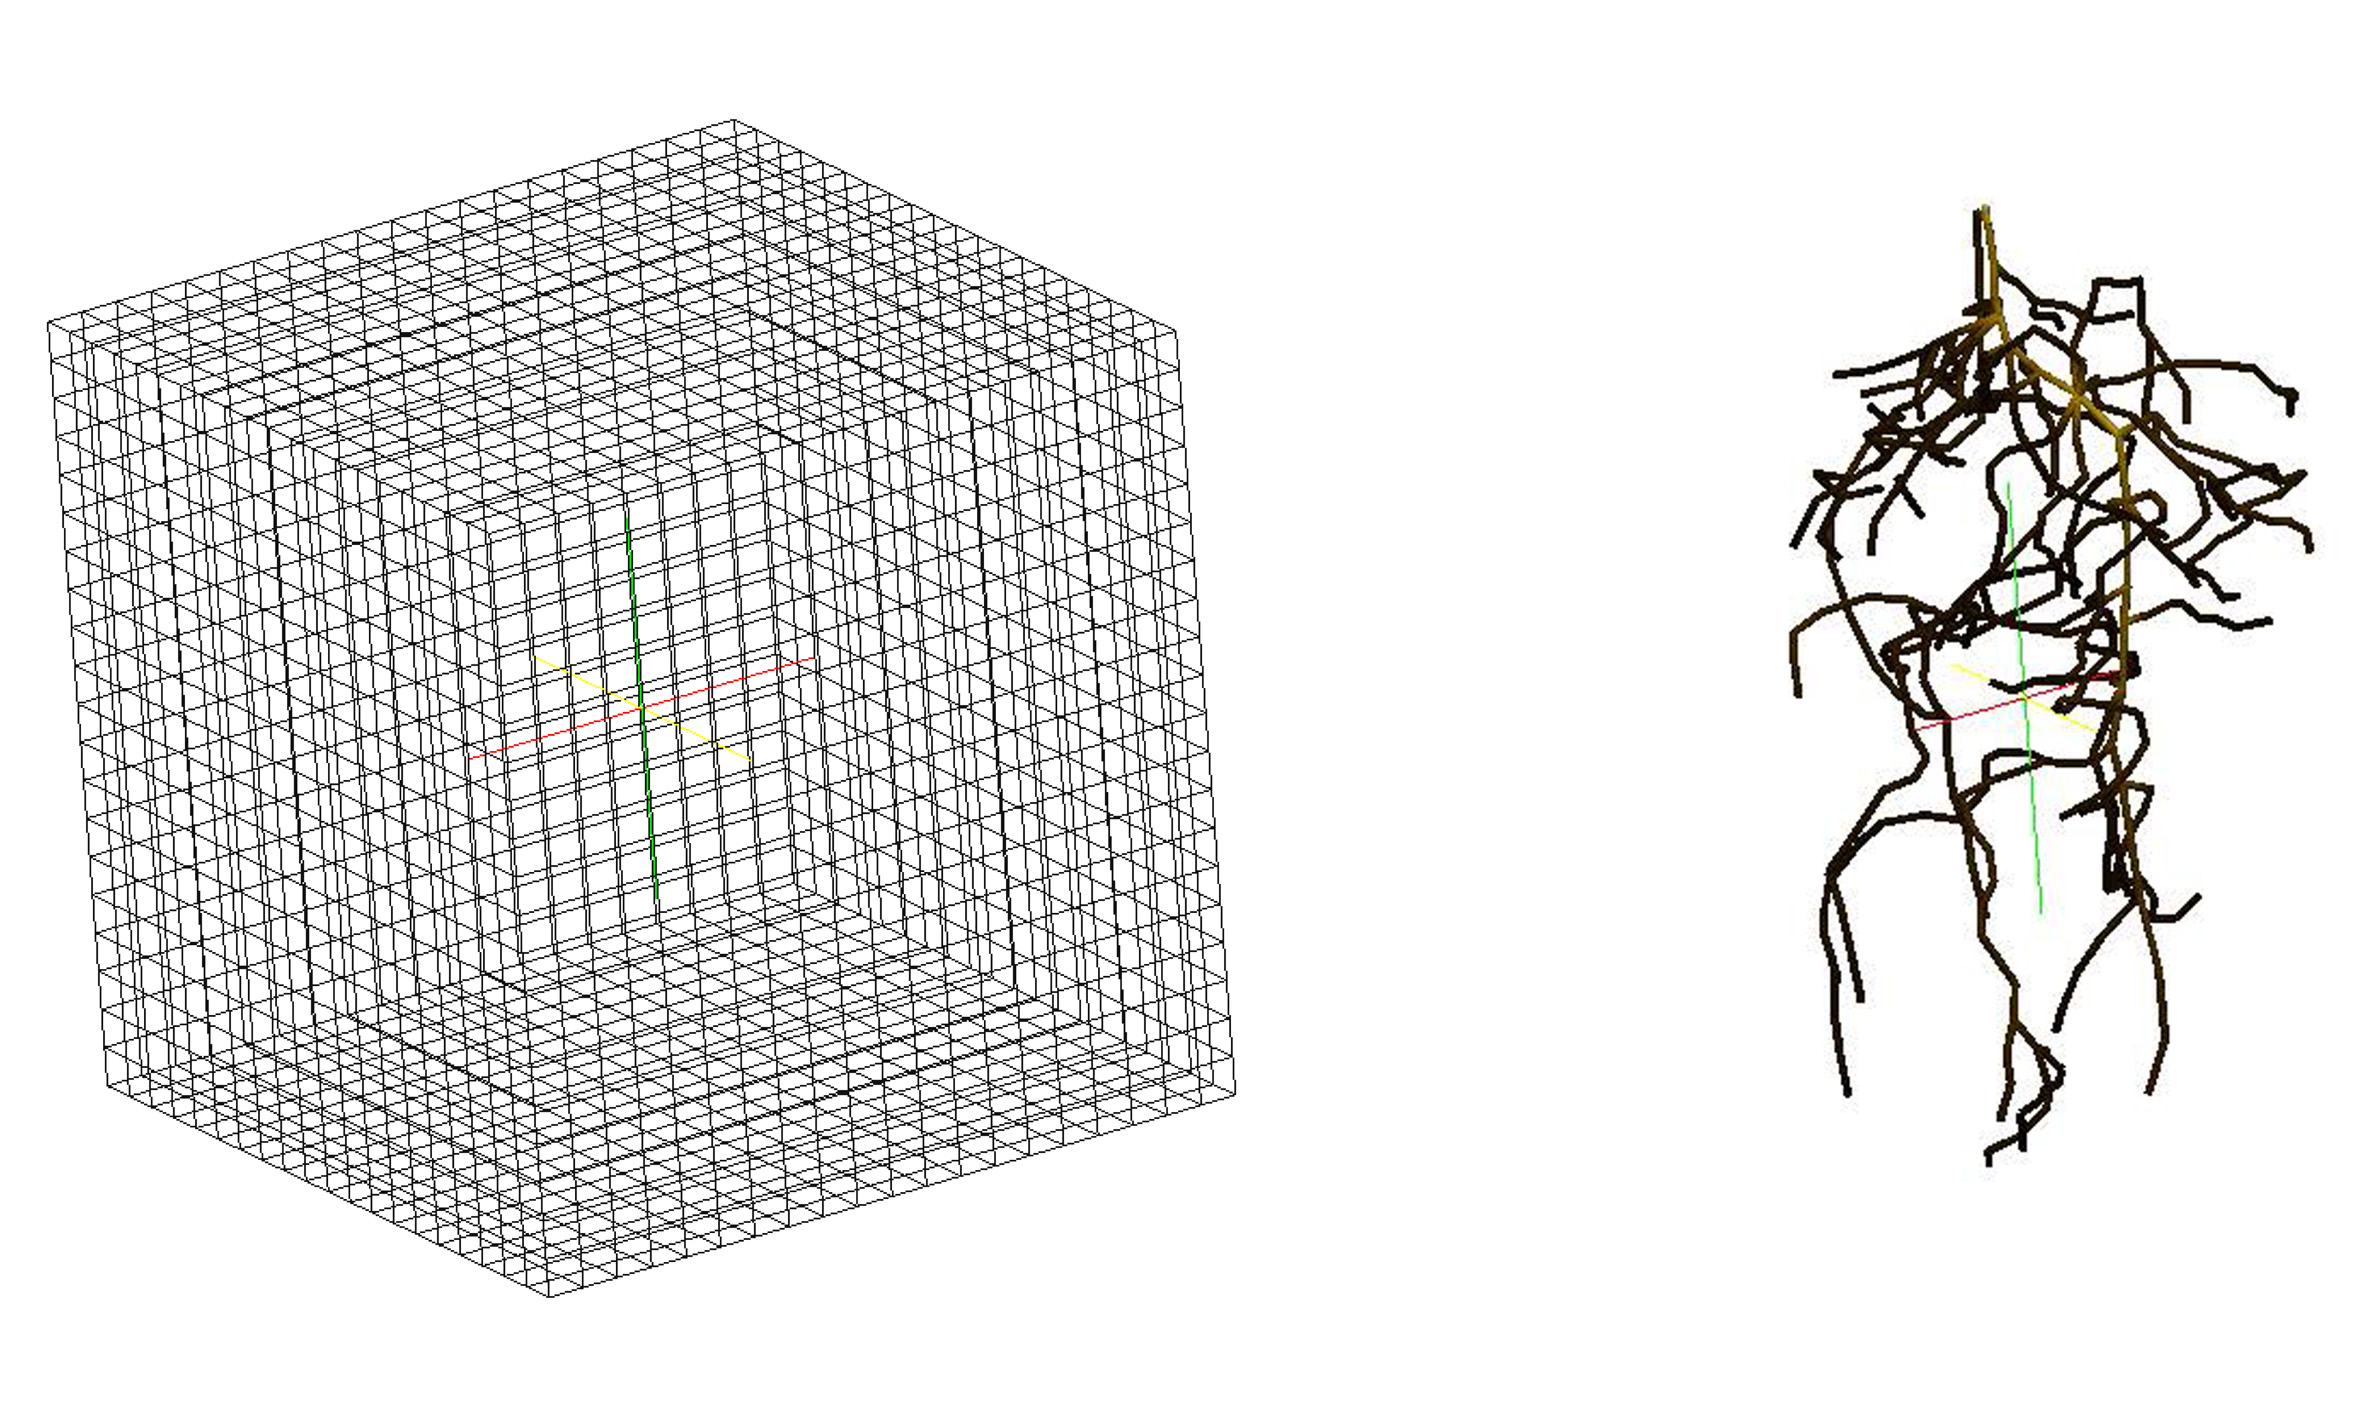
\includegraphics[width=0.5\textwidth]{grids.jpg}
	\caption{The 3D soil grid and the 1D, branched, grid representing the root architecture}
	\label{fig:grids}
\end{figure}

In the example of the coupled problems, both are used simultaneously. In that case, the two grids are merged via source/sink terms in positions where root and soil grids share the same spatial coordinates. This is illustrated in Fig. \ref{fig:merged}; detailed descriptions can be found in the individual examples. 
 
\begin{figure}[ht]
	\centering
  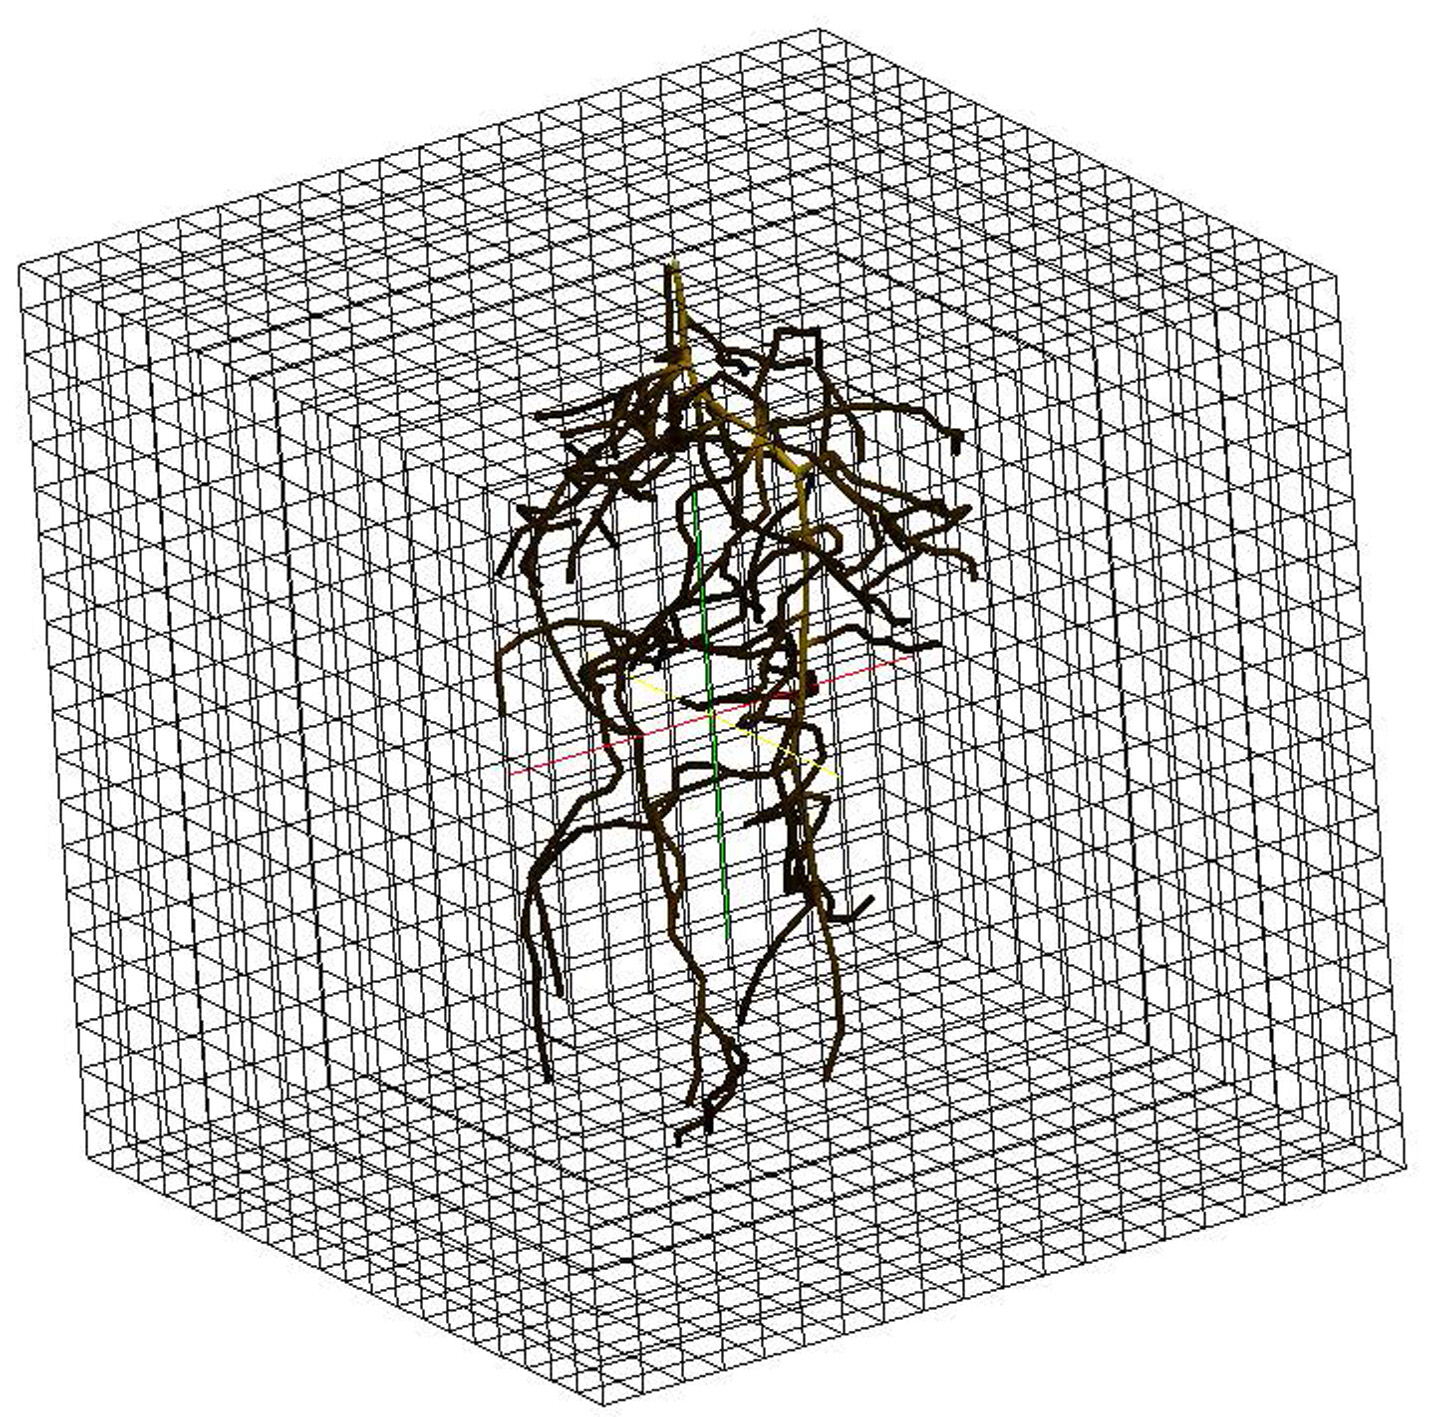
\includegraphics[width=0.33\textwidth]{merged.jpg}
	\caption{3D soil grid merged with the 1D, branched, grid representing the root architecture}
	\label{fig:merged}
\end{figure}

Grids can be created using different DUNE internal or external grid managers (see documentation of dune-grid). In the input file, the details about the numerical grids are specified in the groups [RootSystem.Grid] or [Soil.Grid]. Each folder contains a folder named ``grids" where grids can be provided in dgf format. In the dumux-rosi examples, the soil grid is usually a structured grid created by the default ``GridCreator", where corner points of the domain, spatial resolution and cell type are specified such as in the following example: 

\begin{lstlisting}
[ Grid ]
LowerLeft = 0 0 0
UpperRight = 1 1 1
Cells = 10 10 20
CellType = Cube # or Simplex
\end{lstlisting}

Alternatively, msh-files can be read. 

\section*{Choice of grid manager for the soil domain}
\textbf{YaspGrid}: Structured grids, only non-periodic soil domains\\
\textbf{SpGrid}: Structured grids, also periodic soil domains\\
\textbf{AluGrid}: Unstructured grids, only works for \texttt{CC_2pfa}-scheme\\
\textbf{UGGrid}: Unstructured grids, works for both \texttt{CC_2pfa} and Box schemes\\

Thus, we suggest SPGrid as default grid manager for problems with structured grids and UGGrid as default grid manager for problems with structured grids. 

\section*{How to switch grid manager}
To change the grid manager, open the file \lstinline{dumux-rosi/rosi_benchmarking/coupled_1p_richards/CMakeLists.txt}. If not available, add the following lines to make the gridmanager available to build an executable. For the example of UGGrid:\\

\lstinline{add_executable(coupledUG EXCLUDE_FROM_ALL coupled.cc)}\\
\lstinline{target_compile_definitions(coupledUG PUBLIC DGF GRIDTYPE=Dune:: UGrid<3>)}

\section*{Grids for root systems}

There are two options to specify the root system grid. The first option is to specify it as a file in dgf-format that specifies the coordinates and connection of nodes (verteces).  

\begin{lstlisting}
DGF
Vertex
0 0 -0.03
-0.003301 -0.000687124 -0.0394144
-0.00339314 -0.00159054 -0.0473627
-0.00590116 -0.00546716 -0.0538958
-0.0115931 -0.00454388 -0.059441
-0.0105464 -0.00572357 -0.067284
-0.0100044 -0.0069212 -0.0751753
-0.00923561 -0.00814568 -0.0830435
-0.0100507 -0.00678732 -0.0908851
-0.010965 -0.00608665 -0.0962792
-0.00103059 0.000281757 -0.0413509
0.00284233 0.00172545 -0.0449409
0.00619859 0.00411514 -0.0466909
-6.51815e-05 0.00081926 -0.041154
0.000989275 0.00146981 -0.0404847
-0.00013962 0.00162442 -0.0411274
-0.00376417 0.00152097 -0.0477906
-0.00509243 0.00809897 -0.0472907
-0.00667036 0.0130109 -0.0453872
-0.00784569 0.0163412 -0.0446723
-0.00343402 0.00160078 -0.048867
-0.00272936 0.00153492 -0.0511603
-0.00257298 0.00150318 -0.0517729
-0.00605319 0.00128567 -0.051235
-0.00509341 0.00874088 -0.0479026
-0.0051018 0.00890818 -0.0480774
-0.0105648 -0.00490006 -0.0536398
-0.0155357 -0.00427108 -0.0535009
-0.0187161 -0.00393935 -0.0540514
-0.0129246 -0.00794987 -0.0599204
-0.0158011 -0.0137093 -0.0604436
-0.0159531 -0.0140359 -0.0604843
-0.0103269 -0.00178528 -0.069703
-0.0097869 0.000348939 -0.071026
-0.0101116 -0.00387942 -0.0769314
-0.00866863 -0.0079157 -0.0834016
#
SIMPLEX
parameters 10 # id0, id1, order, branchId, surf[cm2], length[cm], radius[cm], kz[cm4 hPa-1 d-1], kr[cm hPa-1 d-1], emergence time [d], subType, organType 
0 1 0 1 0.314159 1 0.05 0 0 0.253641 1 2
1 2 0 1 0.251327 0.8 0.05 0 0 0.461984 1 2
2 3 0 1 0.251327 0.8 0.05 0 0 0.675409 1 2
3 4 0 1 0.251327 0.8 0.05 0 0 0.894171 1 2
4 5 0 1 0.251327 0.8 0.05 0 0 1.11854 1 2
5 6 0 1 0.251327 0.8 0.05 0 0 1.34882 1 2
6 7 0 1 0.251327 0.8 0.05 0 0 1.58532 1 2
7 8 0 1 0.251327 0.8 0.05 0 0 1.82839 1 2
8 9 0 1 0.17328 0.551569 0.05 0 0 2 1 2
1 10 1 2 0.0591391 0.313743 0.03 0 0 0.81929 2 2
10 11 1 2 0.103194 0.547463 0.03 0 0 1.36938 2 2
11 12 1 2 0.084377 0.447634 0.03 0 0 2 2 2
10 13 2 3 0.0141039 0.112236 0.02 0 0 1.88447 3 2
13 14 2 3 0.0176961 0.140821 0.02 0 0 2 3 2
13 15 3 4 0.0101666 0.080903 0.02 0 0 2 4 2
2 16 1 8 0.0596143 0.316264 0.03 0 0 0.976223 2 2
16 17 1 8 0.126845 0.672936 0.03 0 0 1.39819 2 2
17 18 1 8 0.103656 0.549912 0.03 0 0 1.75726 2 2
18 19 1 8 0.0679195 0.360324 0.03 0 0 2 2 2
16 20 2 9 0.0141835 0.112869 0.02 0 0 1.55953 3 2
20 21 2 9 0.0301593 0.24 0.02 0 0 1.81594 3 2
21 22 2 9 0.00795504 0.0633042 0.02 0 0 2 3 2
20 23 3 10 0.0445473 0.354496 0.02 0 0 2 4 2
17 24 2 12 0.0111449 0.088688 0.02 0 0 1.98626 3 2
24 25 2 12 0.00304236 0.0242104 0.02 0 0 2 3 2
3 26 1 16 0.088687 0.470499 0.03 0 0 1.35817 2 2
26 27 1 16 0.0944815 0.50124 0.03 0 0 1.74414 2 2
27 28 1 16 0.0611608 0.324468 0.03 0 0 2 2 2
4 29 1 19 0.0695225 0.368828 0.03 0 0 1.49515 2 2
29 30 1 19 0.121751 0.645908 0.03 0 0 1.97249 2 2
30 31 1 19 0.00683211 0.0362455 0.03 0 0 2 2 2
5 32 1 22 0.0872183 0.462707 0.03 0 0 1.79818 2 2
32 33 1 22 0.0484141 0.256845 0.03 0 0 2 2 2
6 34 1 24 0.0662369 0.351397 0.03 0 0 2 2 2
7 35 1 25 0.0133627 0.0708913 0.03 0 0 2 2 2
#
BOUNDARYDOMAIN 
default 1
#
\end{lstlisting}

The paragraph ``SIMPLEX" specifies 10 parameters for each root segment: node1ID, node2ID, order, branchID, surfaceIdx in cm$^2$, length in cm , radiusIdx in cm, axialCondIdx cm$^4$ hPa$^{-1}$ d$^{-1}$, radialCondIdx cm hPa$^{-1}$ d$^{-1}$, emergenceTimeId\footnote{Note: in the code we often use the term ´´creation time", however, we always mean ´´emergence time". Branch nodes exist twice, once in the mother branch, once as the starting node of the daughter branch. They have different emergence times but the same nodeID.} Order numbering starts with 0, i.e., primary roots have order 0. Potential artificial shoot segements have order -1. 

Root systems in dgf format can be computed from measured root systems as well as with the root architecture module of CPlantBox. 

The second option is to provide the root architectural parameters in the input file such that the root architecture and related grid is computed by CRootBox while used as a DuMu$^x$ module. 

\begin{lstlisting}
[RootSystem.Grid]
File = Triticum_aestivum_a_Bingham_2011  
InitialT = 10 # days
\end{lstlisting}

Important to know: It is currently necessary to build the code either for option 1 or for option 2 (i.e., two executables can be built that need to be provided with the correct input at runtime). 